%%%%%%%%%%%%%%%%%%%%%%%%%%%%%%%%%%%%%%%%%%%%%%%%%%%%%%%%%
%%             东南大学数电实验报告 LaTeX 模板
%%               Experiment 3 Report.tex
%% https://github.com/Teddy-van-Jerry/SEU_Digital_Report
%% ======================================================
%% 版本信息:
%% v1.0 (Nov. 07, 2021)
%% ------------------------------------------------------
%% 模板制作:
%% Teddy van Jerry, (me@teddy-van-jerry.org)
%% * GitHub: https://github.com/Teddy-van-Jerry
%% * Website: https://teddy-van-jerry.org
%% * Blog: https://blog.teddy-van-jerry.org
%% ------------------------------------------------------
%% 使用说明:
%% 1. 编译使用 XeLaTeX 和 Biber
%% 2. 报告基本信息通过修改导言区以 exp 开头的命令
%% 3. 参考文献位于 ref/ref.bib
%% 4. 报告模板依据 MIT License 开源共享
%% ------------------------------------------------------
%% Copyright 2021 (c) Teddy van Jerry
%%
%% Permission is hereby granted, free of charge, to any
%% person obtaining a copy of this software and
%% associated documentation files (the "Software"), to
%% deal in the Software without restriction, including
%% without limitation the rights to use, copy, modify,
%% merge, publish, distribute, sublicense, and/or sell
%% copies of the Software, and to permit persons to whom
%% the Software is furnished to do so, subject to the
%% following conditions:
%%
%% The above copyright notice and this permission notice
%% shall be included in all copies or substantial
%% portions of the Software.
%% 
%% THE SOFTWARE IS PROVIDED "AS IS", WITHOUT WARRANTY OF
%% ANY KIND, EXPRESS OR IMPLIED, INCLUDING BUT NOT
%% LIMITED TO THE WARRANTIES OF MERCHANTABILITY, FITNESS
%% FOR A PARTICULAR PURPOSE AND NONINFRINGEMENT. IN NO
%% EVENT SHALL THE AUTHORS OR COPYRIGHT HOLDERS BE LIABLE
%% FOR ANY CLAIM, DAMAGES OR OTHER LIABILITY, WHETHER IN
%% AN ACTION OF CONTRACT, TORT OR OTHERWISE, ARISING
%% FROM, OUT OF OR IN CONNECTION WITH THE SOFTWARE OR THE
%% USE OR OTHER DEALINGS IN THE SOFTWARE.
%%%%%%%%%%%%%%%%%%%%%%%%%%%%%%%%%%%%%%%%%%%%%%%%%%%%%%%%%%

%% 使用实验报告模板类(字体大小 11pt 约为五号字)
\documentclass[11pt]{SEU-Digital-Report}

%%%%%%%%%%%%%%%%%%%% 报告基本信息 %%%%%%%%%%%%%%%%%%%%
\expno{六} % 实验序号
\expname{汇编语言程序设计} % 实验名称
\expauthor{赵舞穹} % 姓名
\expID{61520522} % 学号
\expmates{郑瑞琪} % 同组
\expmatesID{61520523} % 学号(同组)
\expmajor{工科试验班} % 专业
\explab{计算机硬件技术} % 实验室
\expdate{2021年12月3日} % 实验日期
\expreportdate{\today} %报告日期
\expgrade{} % 成绩评定
\exptutor{冯熳} % 评阅教师
%%%%%%%%%%%%%%%%%%%%%%%%%%%%%%%%%%%%%%%%%%%%%%%%%%%%

\usepackage{pgfplots}
\pgfplotsset{compat=1.11}
\usepackage[export]{adjustbox} % for figure border

%% 报告正文
\begin{document}
  % 打印封面页
  \exptitlepage

  \tableofcontents
  \newpage

  \section{实验目的}
    \begin{itemize}
      \item 掌握汇编语言源程序设计基本概念,掌握指令和伪指令的基本使用方法,掌握程序
      开发的各个环节—编辑、汇编、链接、调试、运行;
      \item 学习掌握计算机控制台输入输出的基本概念,了解系统调用的概念;
      \item 学习掌握利用QtSpim 工具软件实现MipsR2000 汇编与运行调试功能,加深指令理
      解认识,加深对函数调用、多汇编语言模块组织、多模块间调用/引用方法的认识理
      解,实现Console 输入输出的基本多模块框架;
      \item 学习掌握利用MASM/TASM—Link/Tlink 的汇编环节,学会Debug/TD 调试X86 汇
      编语言程序方法,加深指令宏观理解认识;(课外为主,配合实验7、8 接口技术)\cite{guide}
    \end{itemize}

  \section{实验内容}

    \subsection{汇编语言调试}

      这在上周的实验报告中已经做了详细的介绍,此处将几个重要的点再次说一下.

      MIPS 使用的是 Spim(QtSpim),我更多使用命令行的控制台版本,因为使用方便,创建使用 \texttt{touch file.asm},编辑 \texttt{nano file.asm} 或 \texttt{vim file.asm},\texttt{spim} 进入 Spim 编译器.
      \begin{itemize}
        \item \texttt{reinitialize} 重初始化;
        \item \texttt{load "file.asm"} 导入文件;
        \item \texttt{run <ADDR>} 运行,可选开始时的地址;
        \item \texttt{step <N>} 单步运行,可选运行步数;
        \item \texttt{print} 输出,可以是一个寄存器,如 \texttt{print \$s0},也可以是地址 \texttt{print 0x00400060};
        \item \texttt{exit} 退出.
      \end{itemize}

      X86 测试使用 DOSBox,主要内容见第~\ref{subsec:dosbox}~节.

    \subsection{MIPS 迭代函数}

      \subsubsection{阶乘}

        迭代法求阶乘的代码如图~\ref{subfig:spim_factorial_direct_code}~所示,代码\textcolor{violet}{\textbf{自己编写}},在 \texttt{loop} 至 \texttt{end} 标记之间迭代循环,运行结果如图~\ref{subfig:spim_factorial_direct} 所示,结果存储在寄存器 \texttt{\$s1} 中,使用命令 \texttt{print \$s1} 得到 $7!=5040$ 的计算结果.

        \begin{figure}[htbp]
          \centering
          \subfloat[代码(Nano界面)]{
            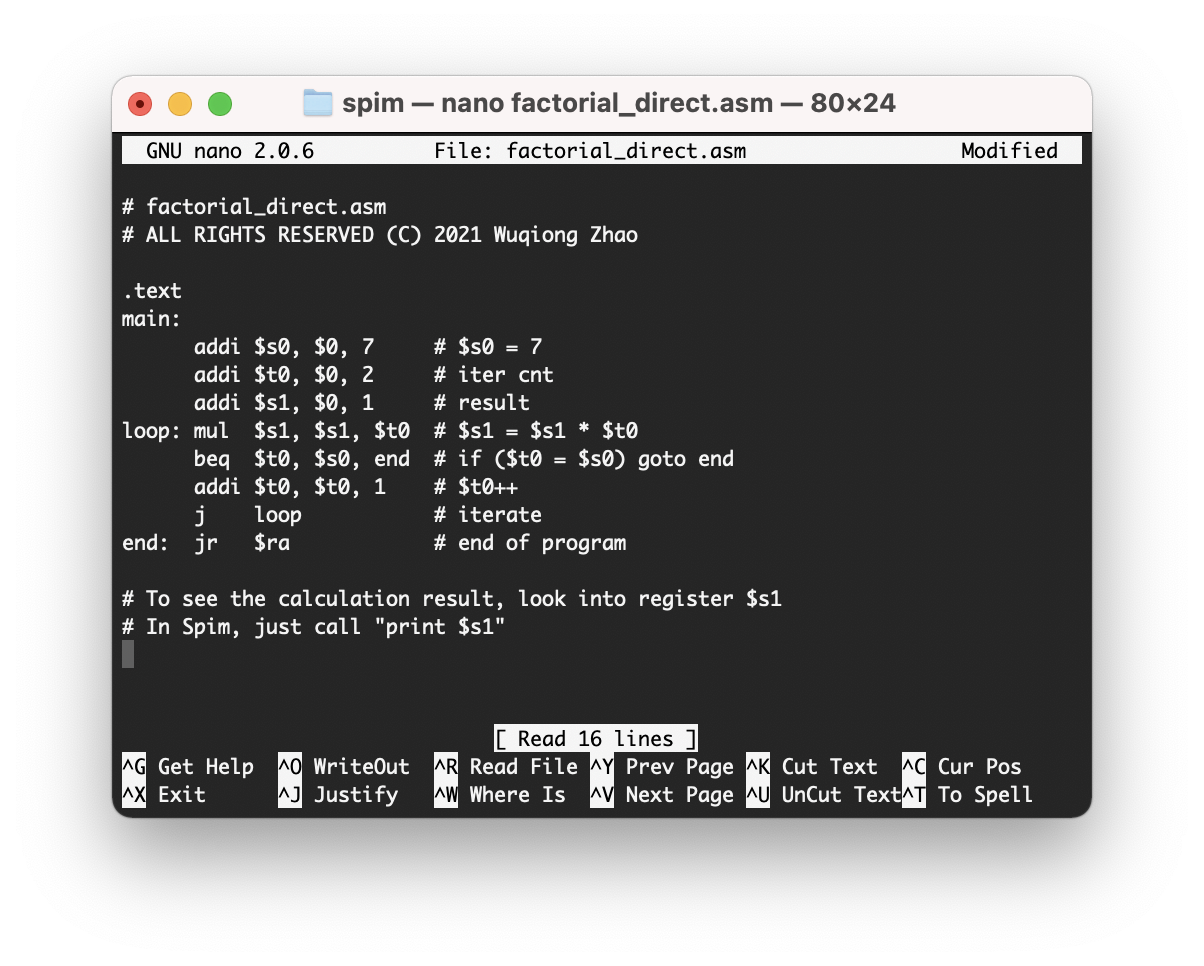
\includegraphics[width=.48\linewidth]{fig/spim_factorial_direct_code.png}
            \label{subfig:spim_factorial_direct_code}
          }
          \subfloat[Spim运行结果]{
            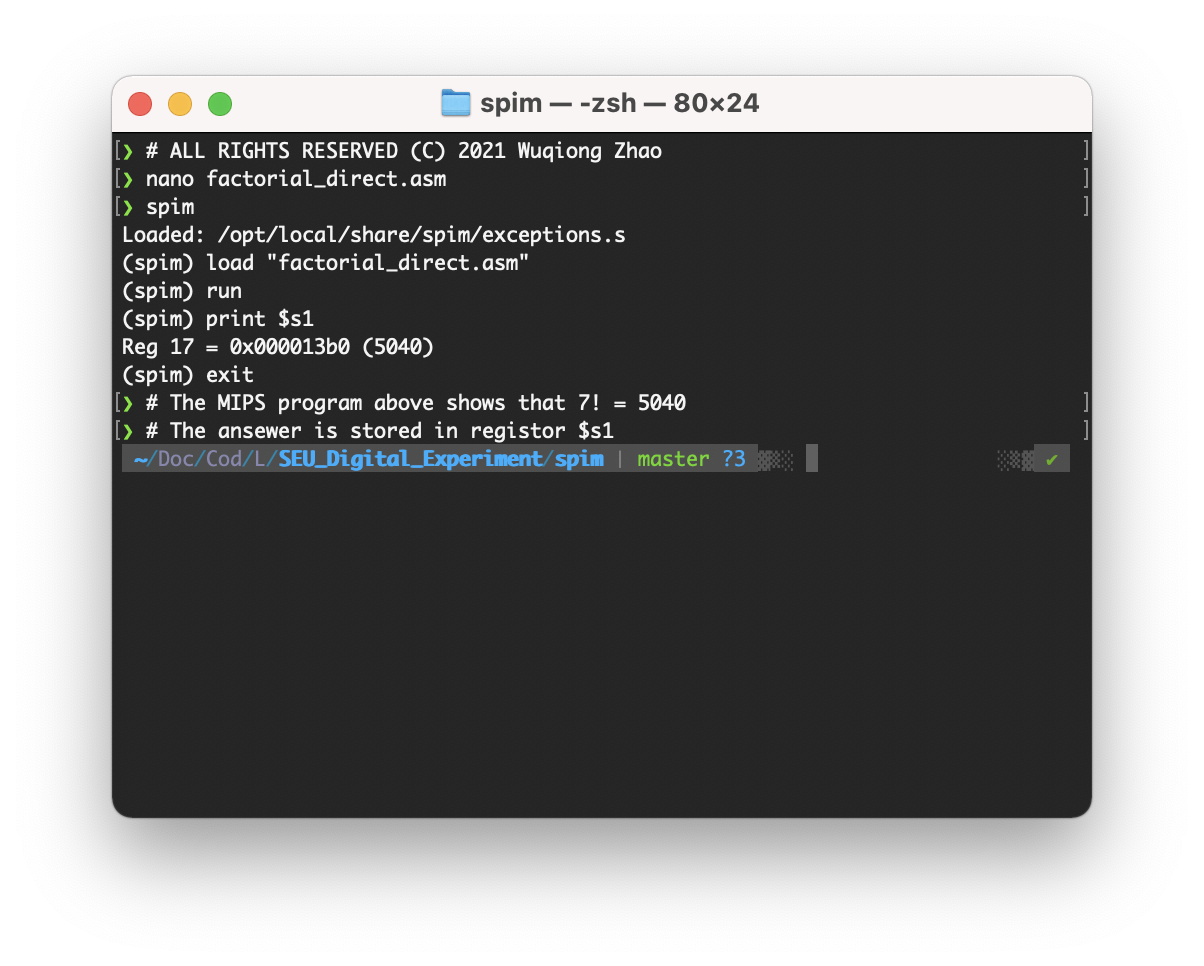
\includegraphics[width=.48\linewidth]{fig/spim_factorial_direct.png}
            \label{subfig:spim_factorial_direct}
          }
          \caption{迭代求阶乘}
          \label{fig:spim_factorial_direct}
        \end{figure}

      \subsubsection{斐波那契数列}

        计算 $100$ 以内最大的斐波那契数.

        修改提供的代码,如图~\ref{subfig:spim_fibonacci_code} 所示,运行结果如图~\ref{subfig:spim_fibonacci} 所示,结果存储在寄存器 \texttt{\$8} 中.

        \newpage

        \begin{figure}[htbp]
          \centering
          \subfloat[代码(Nano界面)]{
            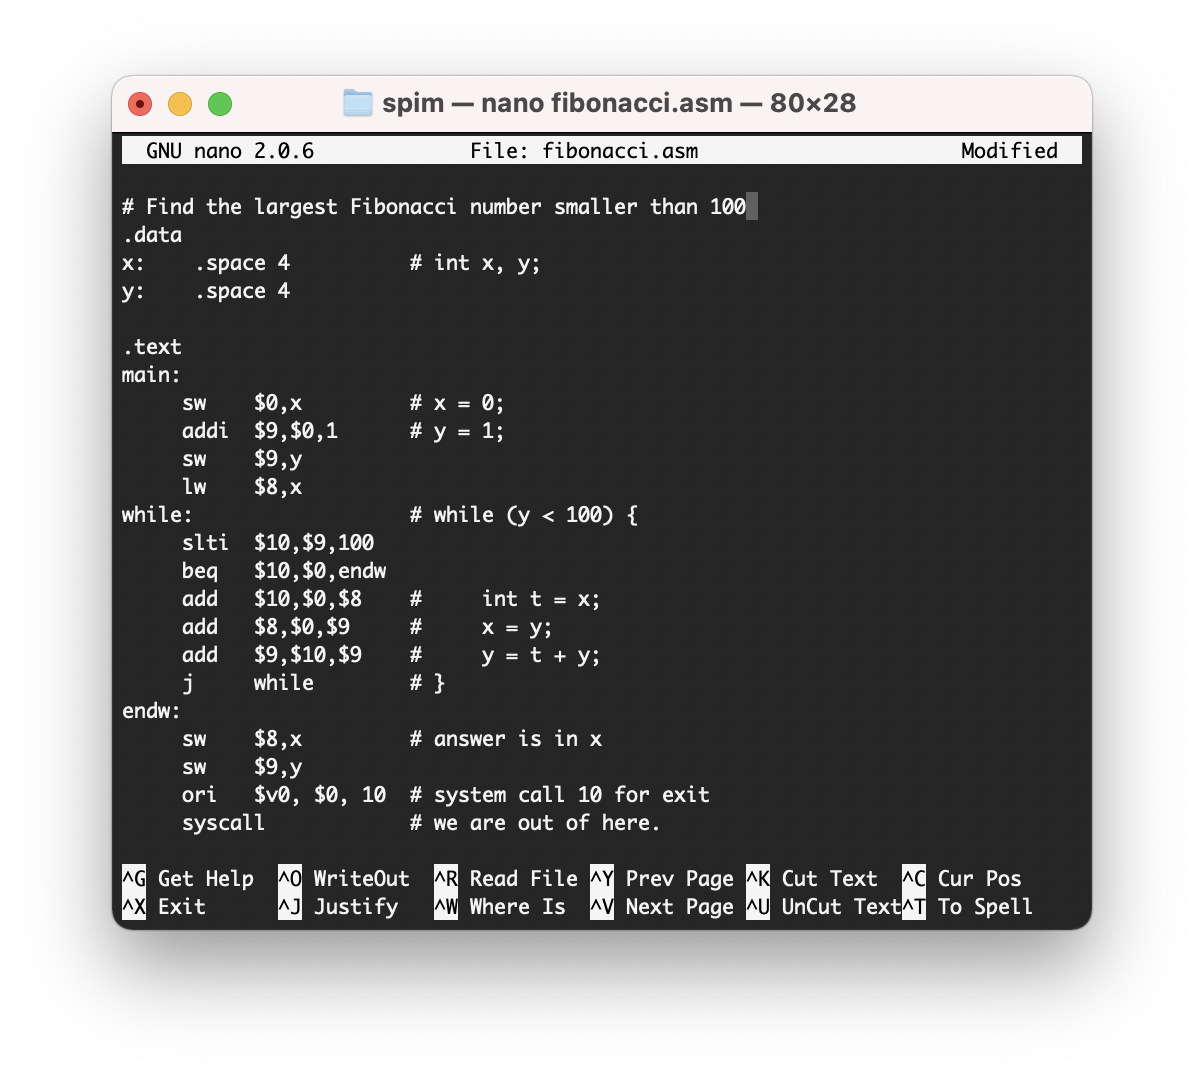
\includegraphics[width=.48\linewidth]{fig/spim_fibonacci_code.png}
            \label{subfig:spim_fibonacci_code}
          }
          \subfloat[Spim运行结果]{
            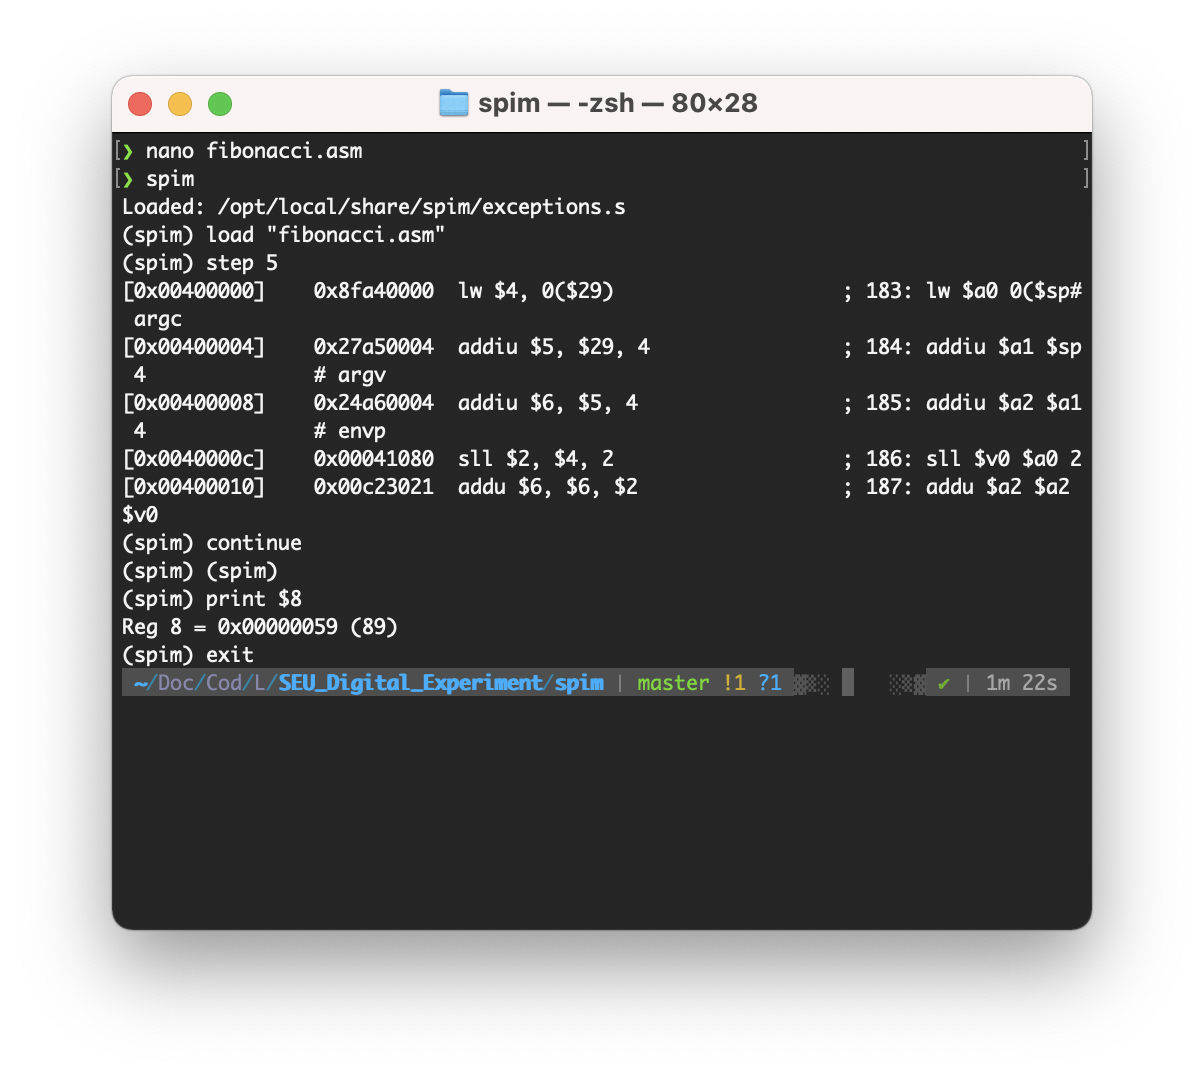
\includegraphics[width=.48\linewidth]{fig/spim_fibonacci.png}
            \label{subfig:spim_fibonacci}
          }
          \caption{迭代求阶乘}
          \label{fig:spim_fibonacci}
        \end{figure}

    \subsection{MIPS 递归函数}

      使用递归的方法计算阶乘.

      编译的 text 结果如图~\ref{subfig:qtspim_text.png}~所示,寄存器 \texttt{\$t1} 中显示结果 \texttt{13b0} 即 $7!=5040$.

      \begin{figure}[htbp]
        \centering
        \subfloat[Text]{
          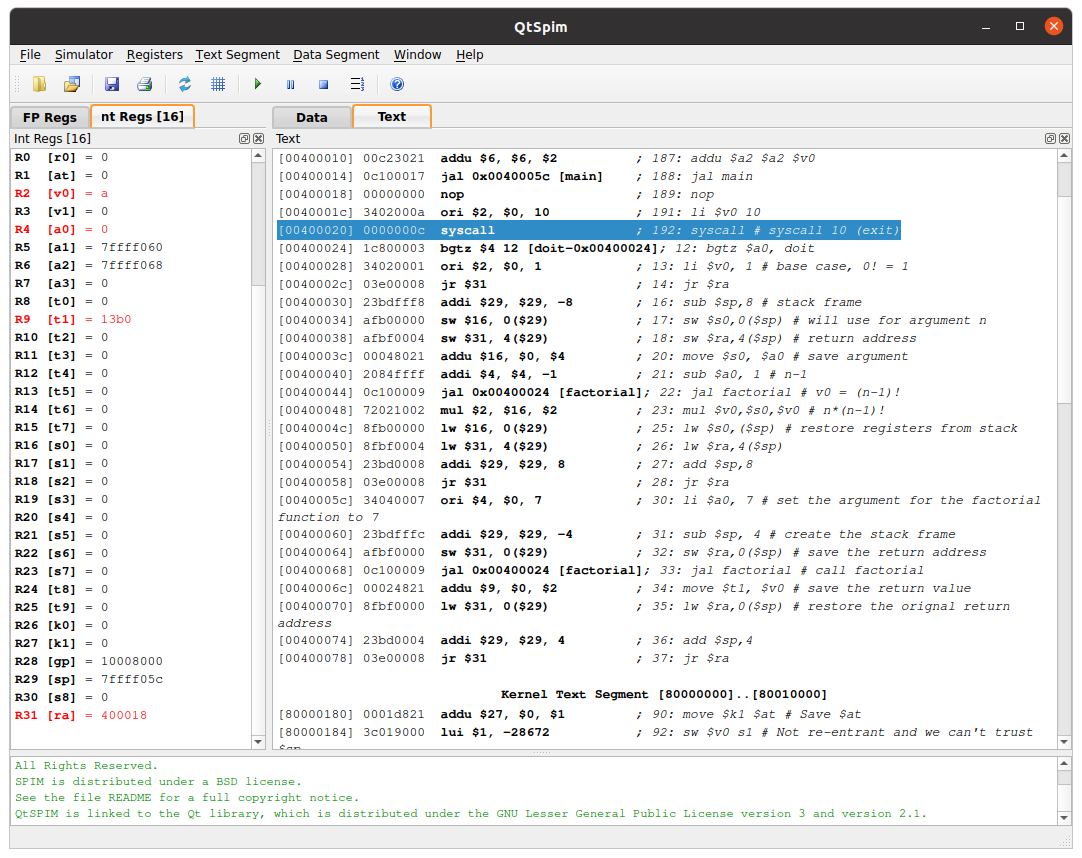
\includegraphics[width=.8\linewidth]{fig/qtspim_text.png}
          \label{subfig:qtspim_text.png}
        } \\
        \subfloat[data]{
          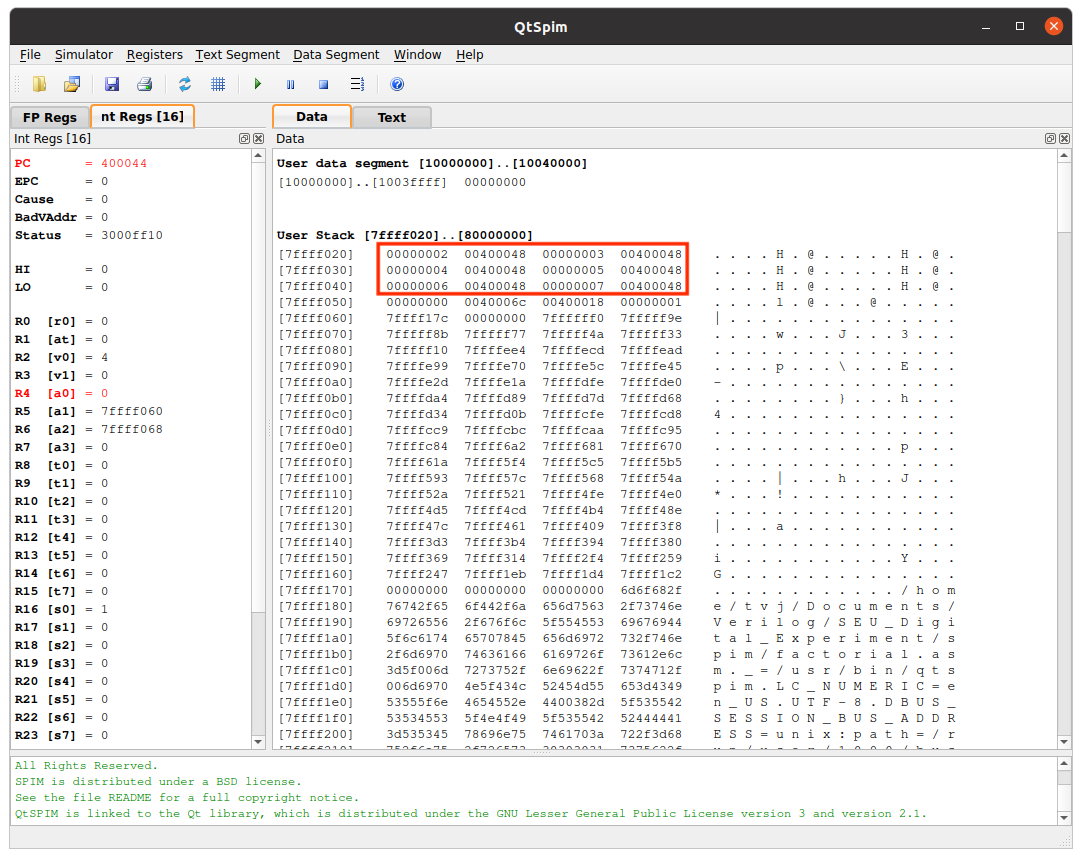
\includegraphics[width=.8\linewidth]{fig/qtspim_data.png}
          \label{subfig:qtspim_data.png}
        }
        \caption{QtSpim}
      \end{figure}

      \begin{analyze}{内存的变化}{}
        内存变化如图~\ref{subfig:qtspim_data.png} 所示,其中红框区域内显示每一次的乘数都被保存.
      \end{analyze}

      \newpage

      我又在提供代码的基础上增加了输入输出,得到了 \texttt{factorial\_pro.asm},
      代码如下,运行结果如图~:
      \begin{lstlisting}[language=sh,tabsize=5,morekeywords={
        j,la,li,syscall,move,sll,sub,bge,sll,add,sw,addi,jal,ls,subu,jr,lw,bgt,bne,lbu,lb,sb,beq,slti,ori
      },title={factorial\_pro.asm}]
# Find the largest Fibonacci number smaller than 100

.data

x:    .space 4          # int x, y;
y:    .space 4
msg1:	.asciiz	"Enter A:   "
msg2:	.asciiz	"Enter B:   "
msg3:	.asciiz	"Largeset Fibonacci No. <100)= "
newline:  .asciiz	"\n"


.text

main:

     sw    $0,x         # x = 0;
     addi  $9,$0,1      # y = 1;
     sw    $9,y
     lw    $8,x

while:                  # while (y < 100) {
     slti  $10,$9,100
     beq   $10,$0,endw
     add   $10,$0,$8    #     int t = x;
     add   $8,$0,$9     #     x = y;
     add   $9,$10,$9    #     y = t + y;
     j     while        # }

endw:
     sw    $8,x         # answer is in x
     sw    $9,y

# Print string msg3
	li	$v0, 4
	la	$a0, msg3
	syscall

	# Print sum
	li	$v0,1         # print_int syscall code = 1
	lw	$a0,x         # int to print must be loaded into $a0
	syscall

	# Print \n
	li	$v0,4         # print_string syscall code = 4
	la	$a0, newline
	syscall


     ori   $v0, $0, 10  # system call 10 for exit
     syscall            # we are out of here.

      \end{lstlisting}

      \begin{figure}[htbp]
        \centering
        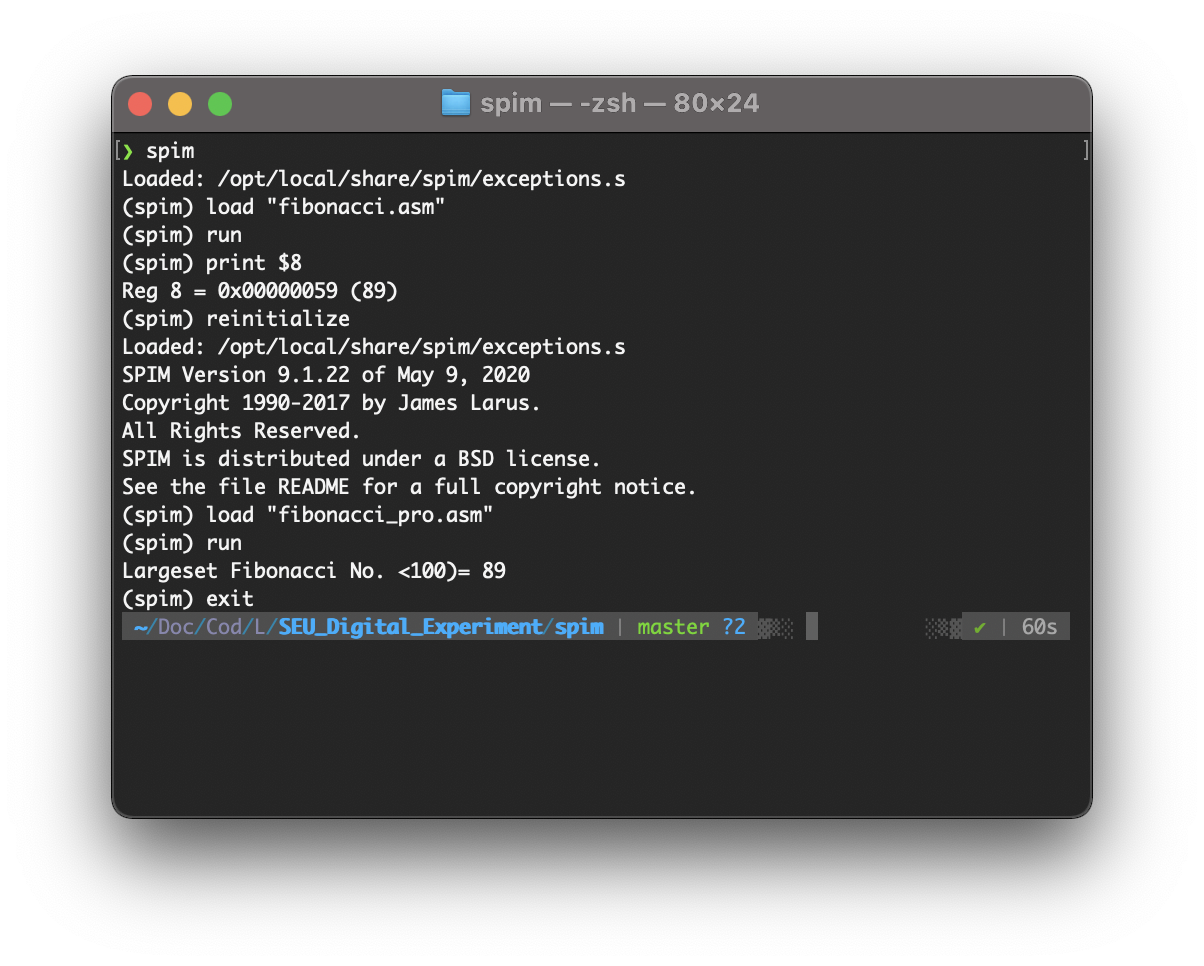
\includegraphics[width=.6\linewidth]{fig/spim_fibonacci_pro.png}
        \caption{\texttt{factorial\_pro.asm}运行结果}
      \end{figure}

    \subsection{MIPS 多模块}

      把\texttt{fact.asm} 作为子模块源程序,主程序\texttt{fact\_main.asm}中\texttt{.extern factorial 32}
      子模块源程序\texttt{.globl fact}说明.

      实现成功,效果如图~\ref{fig:spim_fact} 所示.
      图~\ref{subfig:spim_fact} 中显示,需要将两个文件都 \texttt{load} 才可以,否则会有符号未定义的错误.

      \begin{figure}[htbp]
        \centering
        \subfloat[\texttt{fact.asm} 代码(Nano界面)]{
          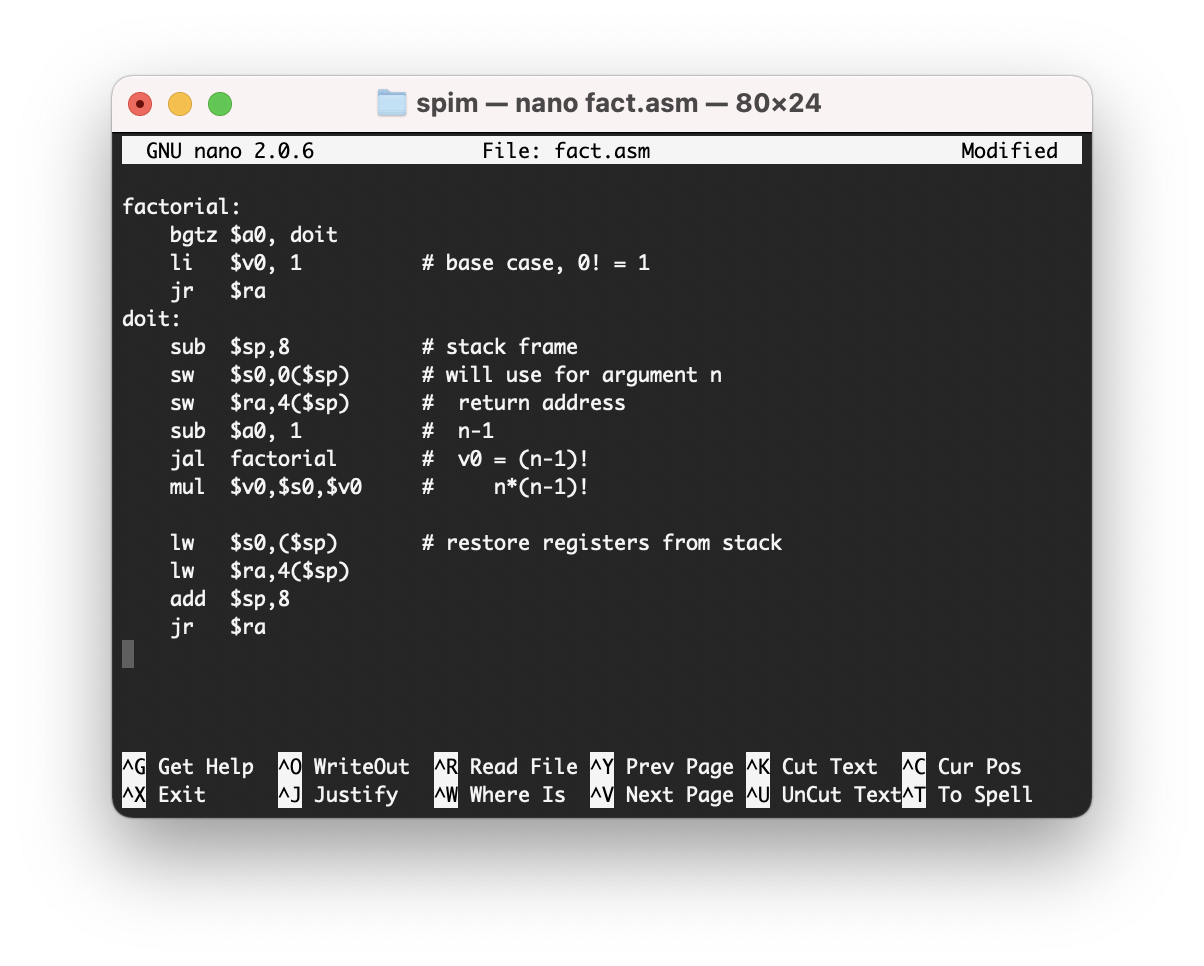
\includegraphics[width=.48\linewidth]{fig/spim_fact_code.png}
          \label{subfig:spim_fact_code}
        }
        \subfloat[Spim运行结果]{
          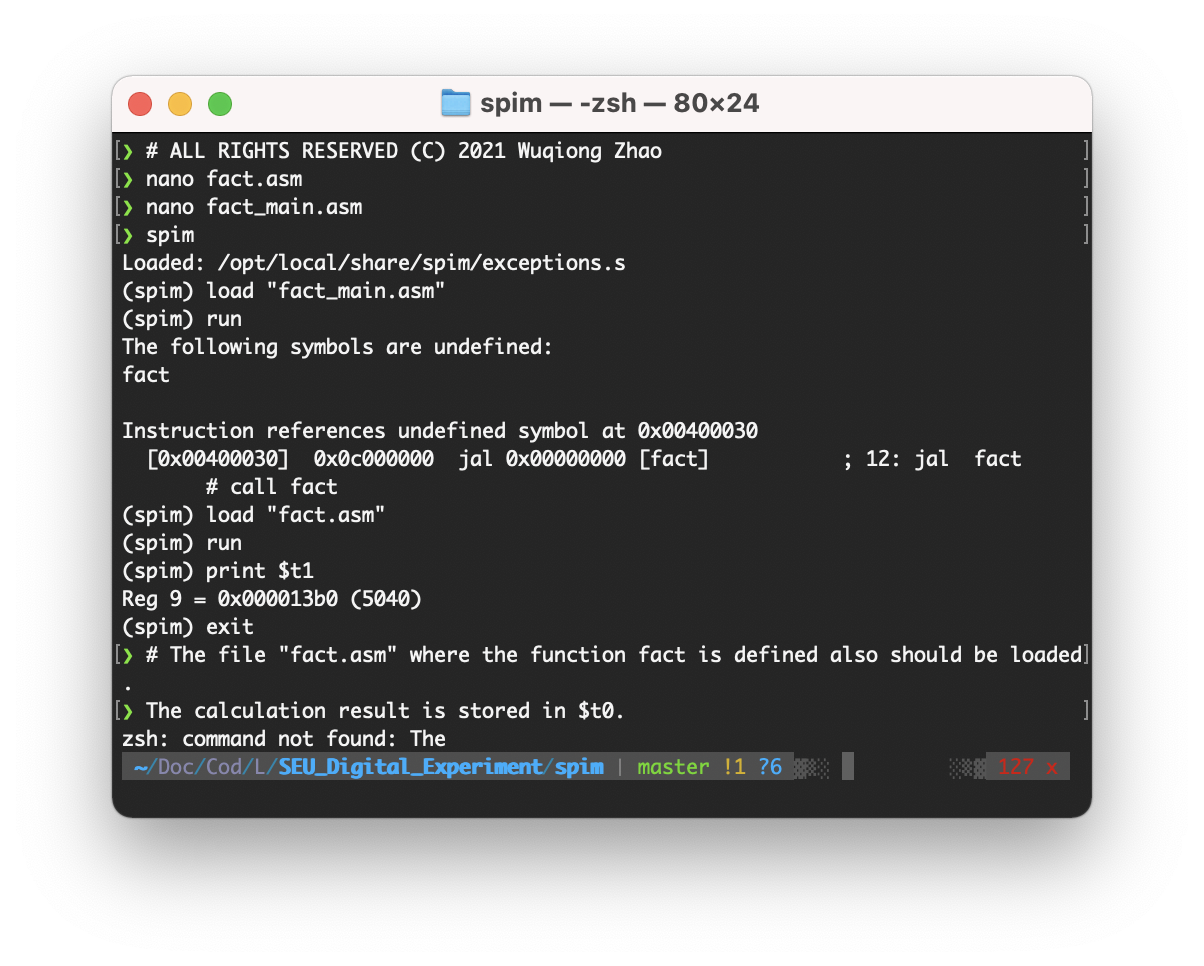
\includegraphics[width=.48\linewidth]{fig/spim_fact.png}
          \label{subfig:spim_fact}
        }
        \caption{迭代求阶乘}
        \label{fig:spim_fact}
      \end{figure}

      \newpage

    \subsection{MIPS 异常处理}\label{subsec:exception}

      首先运行了代码,得到的结果为 $0$ 并且有地址错误,进行 \texttt{step} 调试,关键的步骤如图~\ref{fig:spim_exception_debug} 所示.
      \begin{figure}[h!]
        \centering
        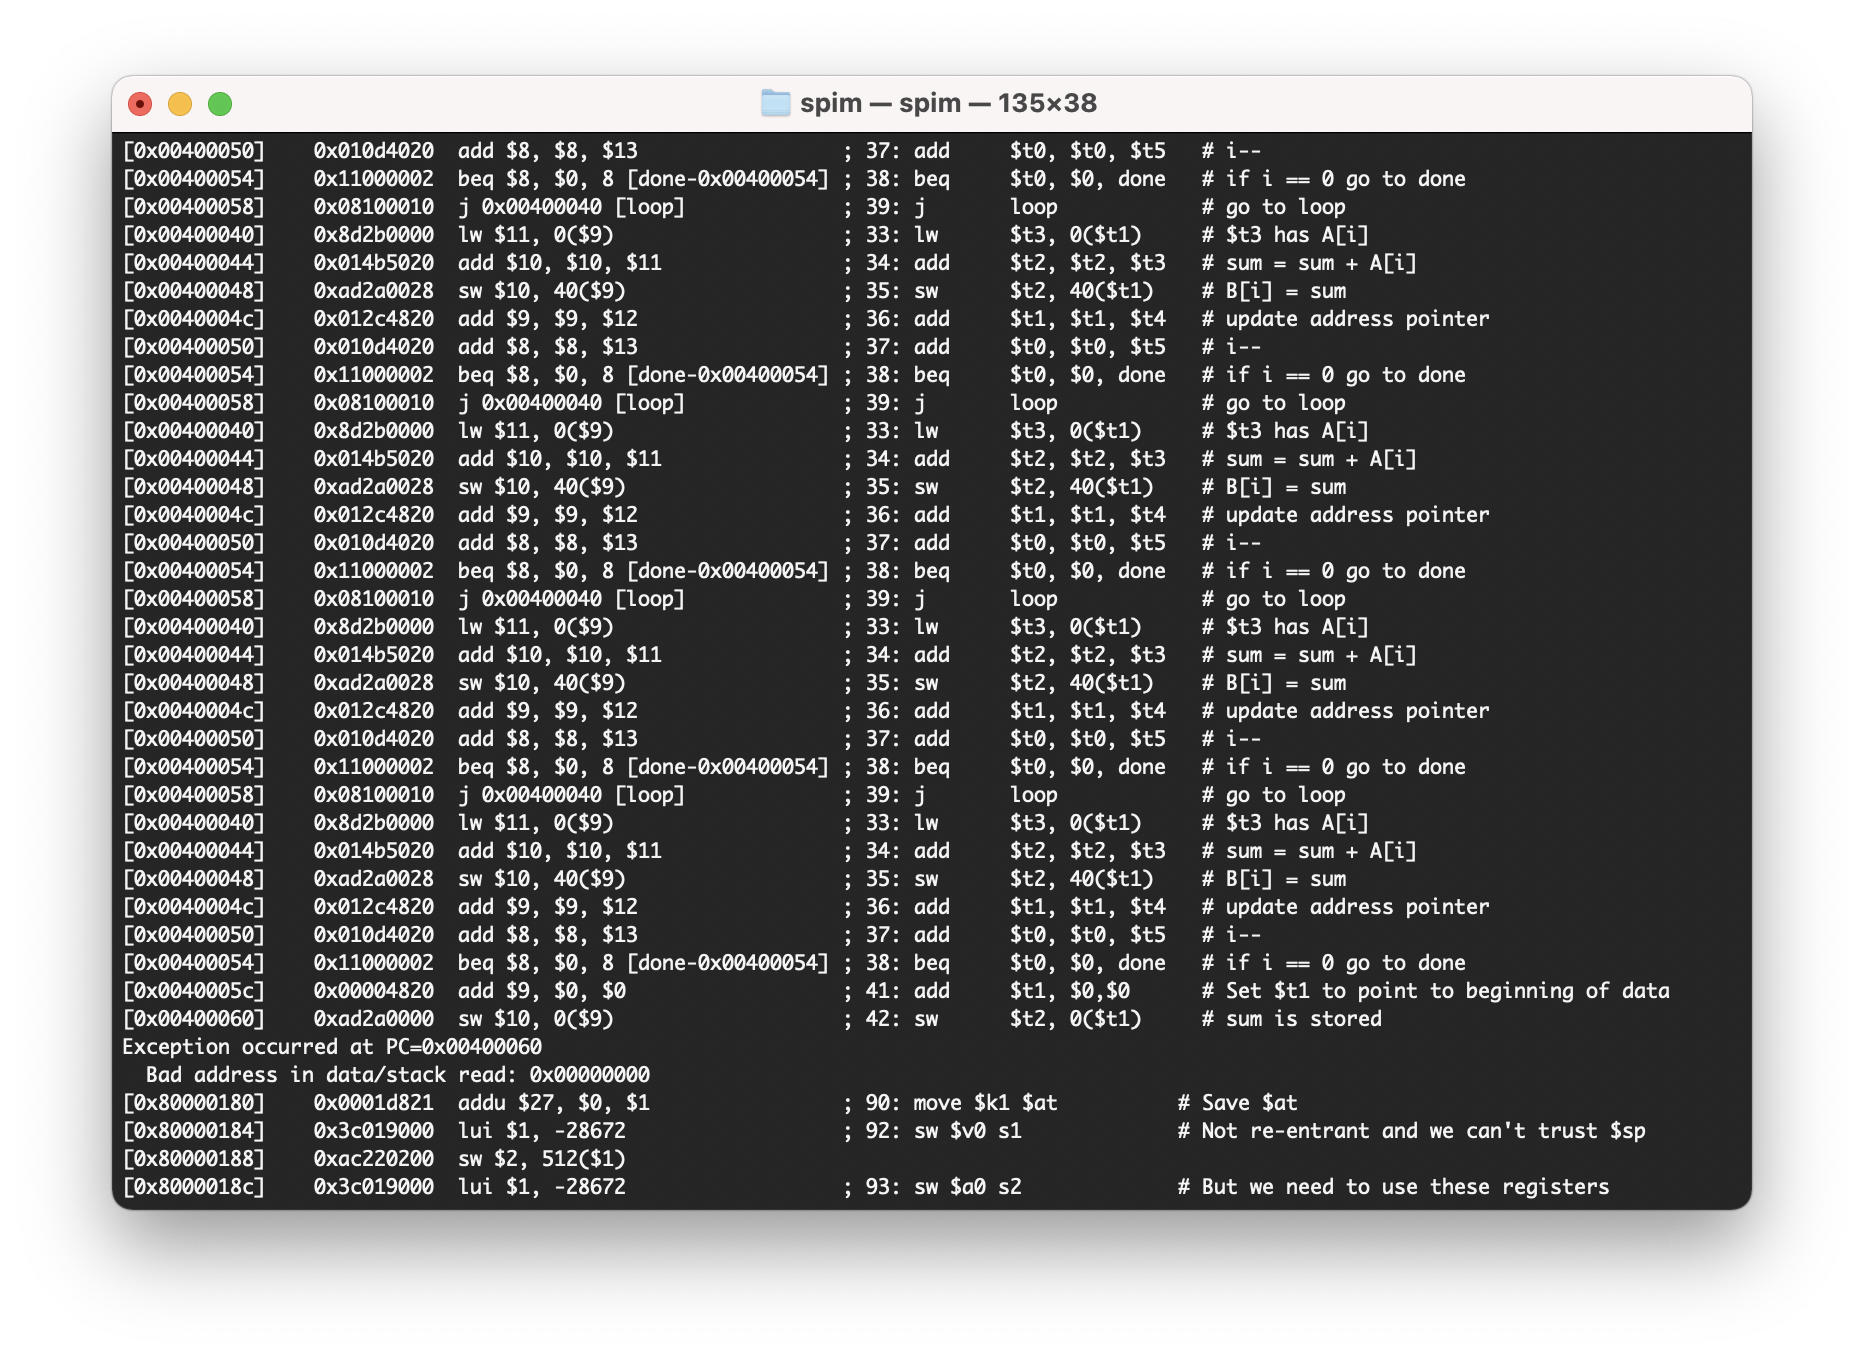
\includegraphics[width=.75\linewidth]{fig/spim_exception_debug.png}
        \caption{\texttt{exception7.s} 调试}
        \label{fig:spim_exception_debug}
      \end{figure}

      \begin{analyze}{\texttt{exception7.s} 异常处理}{}      
        从图~\ref{fig:spim_exception_debug} 中可以看到几个不对的地方,
        第一,跳转 \texttt{loop} 仅有8次,加上第一次进入也只有9次,此外,使用命令 \texttt{print \$t2} 可以得到结果 $36$,而这个值恰好是 $\sum_{i=0}^8i$,因此我们可以认为迭代循环次数存在问题.
        将其修改后问题仍然没有解决,我不使用地址指针,而是直接使用寄存器 \texttt{\$t2} 的值,可以得到正确的结果 \texttt{45},如图~\ref{fig:spim_exception_solve} 所示.
        \begin{center}
          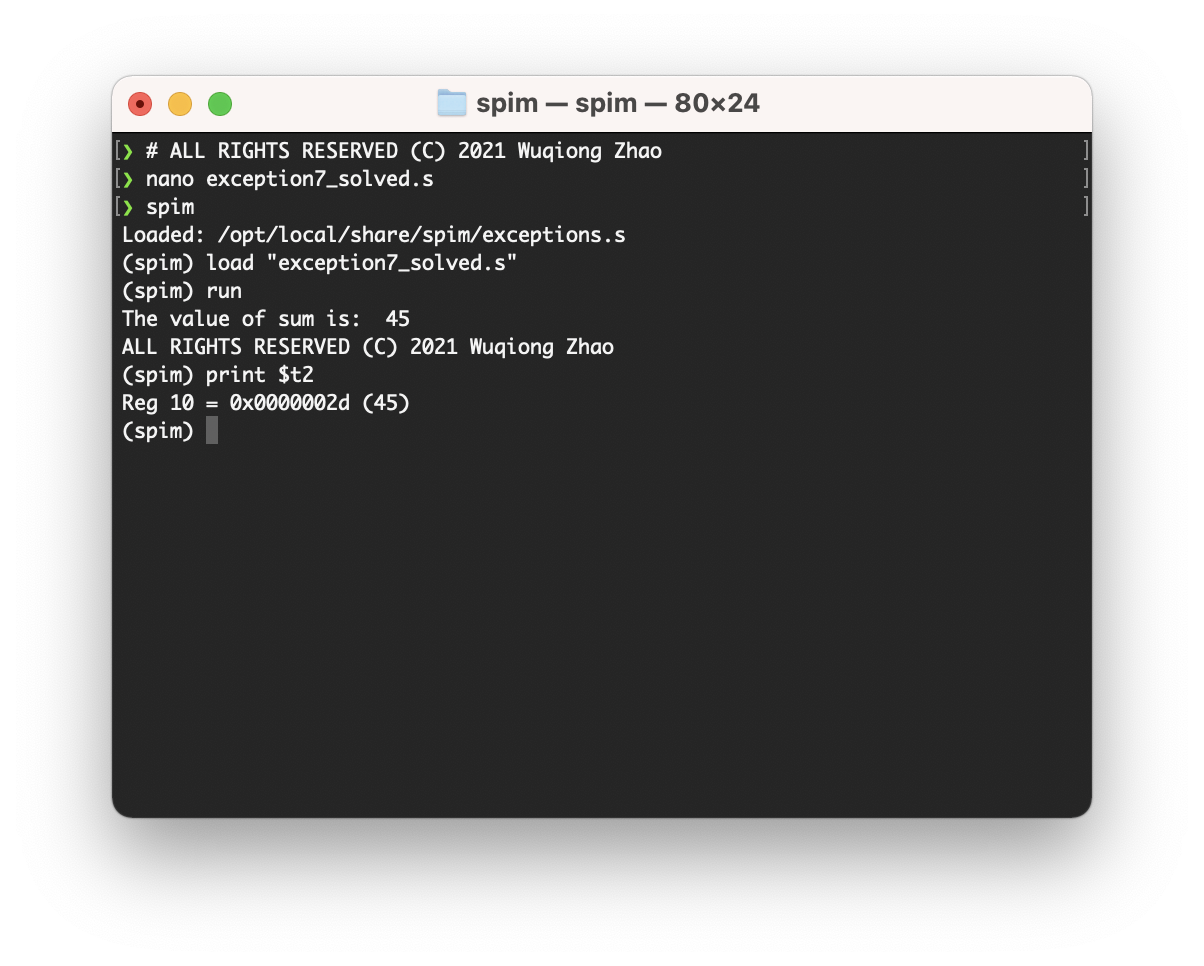
\includegraphics[width=.65\linewidth]{fig/spim_exception_solve.png}
          \captionof{figure}{修改后成功运行的代码输出}
          \label{fig:spim_exception_solve}
        \end{center}
        此外也可以观察到寄存器 \texttt{\$t2} 中的值也是 $45$.
      \end{analyze}

      修改后的代码:
      \begin{lstlisting}[language=sh,tabsize=8,morekeywords={
        j,la,li,syscall,move,sll,sub,bge,sll,add,sw,addi,jal,ls,subu,jr,lw,bgt,bne,lbu,lb,sb,beq,slti,ori
      },title={exception7\_solved.asm}]
# Program for Laboratory 6: Exception Handling
#    This program generates exception number 7 by referring to an address
#    which is out of range
# Implements:
#      sum = 0;
#      i = 9;
#   do {
#      sum = sum + A[9-i]
#      B[9-i] = sum;
#      i--;
#   until (i == 0)

# Sloved by 61520522 Wuqiong Zhao

        .data
sum:    .word   0
A:      .word   0, 1, 2, 3, 4, 5, 6, 7, 8, 9
B:      .word   10, 11, 12, 13, 14, 15, 16, 17, 18, 1
Four:   .word   4
Nine:   .word   9
Minus1: .word   -1
msg:    .asciiz "The value of sum is:  "
notice: .asciiz "\nALL RIGHTS RESERVED (C) 2021 Wuqiong Zhao\n"

        .text
        .globl main
main:
        add     $t2, $0, $0     # sum = 0  (sum is in $t2)
        add     $t1, $0, $0     # Set $t1 to point to beginning of data,
        la      $t1,sum         # that is, to sum
        lw      $t4, 84($t1)    # Constant 4 stored in $t4
        lw      $t0, 88($t1)    # Constant 9 stored in $t0 (i)
        lw      $t5, 92($t1)    # Constant -1 stored in $t5
        add     $t1, $t1,$t4    # A starts at 4 (move $t1 to point to A)
loop:
        lw      $t3, 0($t1)     # $t3 has A[i]
        add     $t2, $t2, $t3   # sum = sum + A[i]
        sw      $t2, 40($t1)    # B[i] = sum
        add     $t1, $t1, $t4   # update address pointer
        ###### EDIT HERE ########
        beq     $t0, $0, done   # if i == 0 go to done
        add     $t0, $t0, $t5   # i--
        #########################
        j       loop            # go to loop
done:
        #### DELETE TWO LINES ###
        li      $v0, 4          # print_str
        la      $a0, msg
        syscall
        li      $v0, 1          # print_int
        ###### EDIT HERE ########
        move    $a0, $t2
        syscall
        #########################
        
        ###### EDIT HERE ########
        li      $v0,4           # print_string
        la      $a0, notice     # print copyright notice
        syscall
        #########################
        jr      $ra             # return to main

      \end{lstlisting}

    \subsection{X86 编译}\label{subsec:dosbox}

      我编译了一个输出日期时间的汇编程序.
      在正式开始之前,我先配置了 DOSBox 的环境:
      \begin{lstlisting}
mount C: ~/Programmes/DOSBox
mount D: ~/Documents/LaTeX/SEU_Digital_Experiment/dosbox
path C:;D:
      \end{lstlisting}
      然后使用 \texttt{MASM} 和 \texttt{LINK} 先生成 \texttt{obj} 文件再编译成 \texttt{exe} 文件,过程如图~\ref{fig:dosbox} 所示.

      \begin{figure}[htbp]
        \centering
        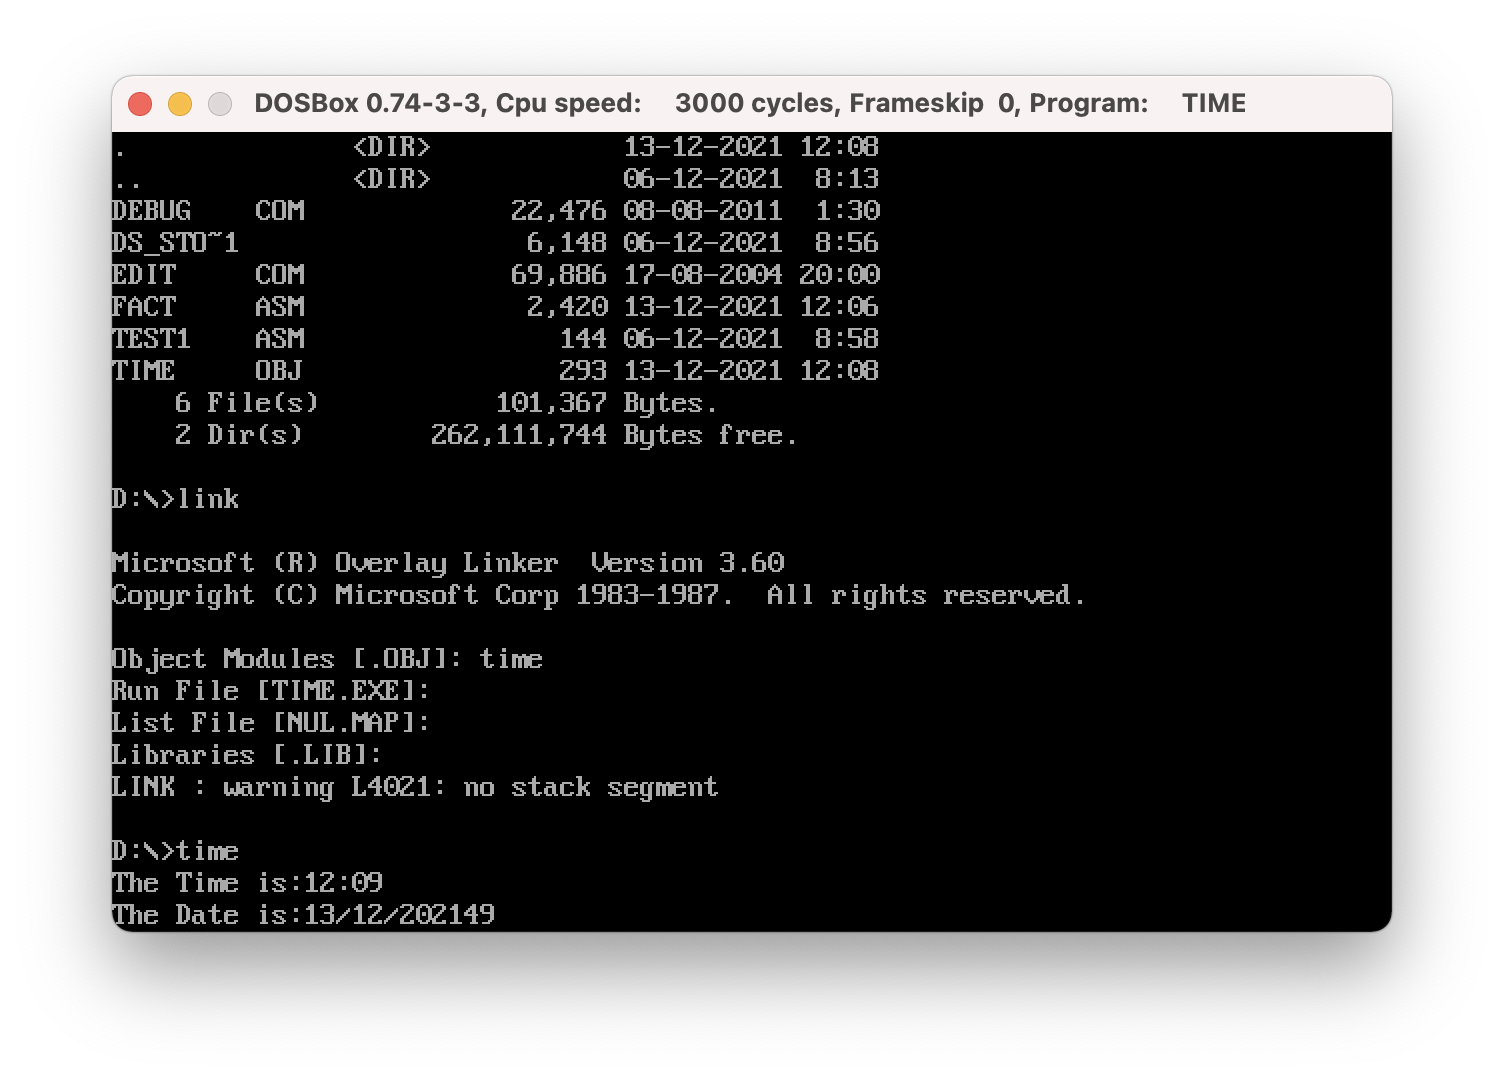
\includegraphics[width=.6\linewidth]{fig/dosbox.png}
        \caption{X86 DOSBox 编译}
        \label{fig:dosbox}
      \end{figure}

  \section{创新与提高}

    首先,我完成了第~\ref{subsec:exception} 节的异常解决工作,成功通过 Spim 命令行完成.

    另外,我也对 MIPS 中数据类型转换做了相应的研究,有以下的代码,将 \texttt{double} 转为 \texttt{int} 型.
    \begin{lstlisting}[language=sh,tabsize=4,morekeywords={
      l,s,d,mtc1,cvt,w,div,mfc1
    },title={convert\_type.asm}]
.data

number: .double 1.3

.text

l.s $f2, number

main:
    l.d     $f0, fp1
    l.d     $f1, fp2

    mtc1    $a0, $f1
    cvt.d.w $f1, $f1
    div.d   $f3, $f1, $f2
    cvt.w.d $f3, $f3
    mfc1    $s2, $f3

    \end{lstlisting}
    
  \section{实验总结}

    这次的实验包括了 MIPS 和 X86 平台汇编代码的训练,整体来说较为简单,是基于一定的训练,有了较高的熟练度,可以像 C++ 一样结合互联网完成所要达成的代码目的.
    说一些感性的内容,我其实非常喜欢汇编语言的样子,非常的简洁(当然只是每一句话,整体必然会很长),配上命令行简直是绝配.
    我们现在写代码基本不会使用汇编,但是任何的编译性语言都基于了汇编,我在写 C++ 的时候就会思考我的代码究竟应该怎样才能优化更多.

    \begin{device}{}{devices}
      \begin{itemize}
        \item QtSpim 9.1.21/22
        \item Spim 8.0 (For Ubuntu), Spim 9.1.22 (For MacOS) {\kaishu\color{gray}(无桌面版本)}
        \item DOSBox 0.74-3-3
        \item Ubuntu 20 (X86\_64) / Windows 11 (X86\_64) / MacOS Big Sur (M1 chip){\kaishu\color{gray}(QtSpim 实验于 Ubuntu 和 MacOS 上完成,DOSBox 于 MacOS 上完成)}
        \item Debian GNU/Linux 10 X86\_64 {\kaishu\color{gray}(TVJ MIPS 的服务器)}
      \end{itemize}
    \end{device}
    

    % 打印参考文献
    \addcontentsline{toc}{section}{参考文献}
    \printbibliography[sorting=none]

    \newpage
    \addcontentsline{toc}{section}{附录 A:实验报告 \LaTeX 模板}
    \section*{附录 A:实验报告 \LaTeX 模板}

        实验报告使用自己编写的 \LaTeX 模板(\texttt{SEU-Digital-Report.cls}),
        在基本适配 Microsoft Word 版报告的格式要求之外,
        增加了更多的功能,使得报告看起来更加优雅多彩.

        后续升级后,报告模板将于 \url{https://github.com/Teddy-van-Jerry/TVJ-Digital-Report} 基于 MIT License 开源共享.

        编译需要使用 \texttt{XeLaTeX + Biber},封面页修改如下内容即可.
        \begin{lstlisting}[
          language=tex,
          morekeywords={
            expno,
            expname,
            expauthor,
            expID,
            expmates,
            expmatesID,
            expmajor,
            explab,
            expdate,
            expreportdate,
            expgrade,
            exptutor,
            today
          }
        ]
%% 使用实验报告模板类(字体大小 11pt 约为五号字)
\documentclass[11pt]{SEU-Digital-Report}

%%%%%%%%%%%%%%%%%%%% 报告基本信息 %%%%%%%%%%%%%%%%%%%%
\expno{五} % 实验序号
\expname{计算机系统与指令认识} % 实验名称
\expauthor{赵舞穹} % 姓名
\expID{61520522} % 学号
\expmates{郑瑞琪} % 同组
\expmatesID{61520523} % 学号(同组)
\expmajor{工科试验班} % 专业
\explab{计算机硬件技术} % 实验室
\expdate{2021年11月26日} % 实验日期
\expreportdate{\today} %报告日期
\expgrade{} % 成绩评定
\exptutor{冯熳} % 评阅教师
%%%%%%%%%%%%%%%%%%%%%%%%%%%%%%%%%%%%%%%%%%%%%%%%%%%%
        \end{lstlisting}

    \addcontentsline{toc}{section}{附录 B:程序真伪判别}
    \section*{附录 B:程序真伪判别}

    \begin{enumerate}
      \item QtSpim 我在报告中使用 Ubuntu 20(GNOME桌面) 和 MacOS Big Sur,窗口非常具有标志性;
      \item Ubuntu 和 MacOS 的 Terminal 我加有注释 \texttt{\# 61520522 Wuqiong Zhao} 和 \texttt{ALL RIGHTS RESERVED (C) 2021 Wuqiong Zhao};
      \item DOSBox 使用 MacOS,并且其中的文件日期 \texttt{13-12-2021} 即报告撰写日期.
    \end{enumerate}

\end{document}
